% Copyright 2020 by Junwei Wang <i.junwei.wang@gmail.com>
%
% This file may be distributed and/or modified under the
% conditions of the LaTeX Project Public License, either version 1.3c
% of this license or (at your option) any later version.
% The latest version of this license is in
%   http://www.latex-project.org/lppl.txt

% \documentclass[aspectratio=169,compress]{beamer}
\documentclass[aspectratio=169,compress]{beamer}

\usepackage[english]{babel}
\usepackage{metalogo}
\usepackage{listings}
\usepackage{fontspec}
\usepackage{tikz}

% \usetheme{Nord}
\usetheme[style=light]{Nord}


%\usepackage[spanish, es-tabla]{babel}
\usepackage[utf8]{inputenc}
\usepackage{hyperref}




\setmainfont{Yanone Kaffeesatz}
%\setsansfont{Andika New Basic}
\setmonofont{DejaVu Sans Mono}

\setbeamerfont{frametitle}{parent=structure,size=\Large}

\AtBeginSection[]
{
  \begin{frame}[c,noframenumbering,plain]
    \tableofcontents[sectionstyle=show/hide,subsectionstyle=show/show/hide]
  \end{frame}
}

\AtBeginSubsection[]
{
  \begin{frame}[c,noframenumbering,plain]
    \tableofcontents[sectionstyle=show/hide,subsectionstyle=show/shaded/hide]
  \end{frame}
}

\title{Arquitecturas y Organización de Computadoras I}
\subtitle{1: Abstracciones en la computadora y tecnología}
\author{Rafael Ignacio Zurita}
\institute{Depto. Ingeniería de Computadoras}
\date{\today}

\begin{document}

\begin{frame}[plain,noframenumbering]
\bigskip
  \maketitle
\end{frame}

% video
% mostrar varias computadoritas
% mostrar placa con integrados y pcb
% mostrar foto de chip y hablar de los transistores
% mostrar imagen wakerly de transistor CMOS

% imagenes 
% foto de performance
% cuadro python vs C
% foto eras tecnologicas

% historia de ibm
% fotos de computadoras hitos
%     ibm 360 (mainframe), cray1 (supercoputaodra)
%     pdp-11 (creacion de unix) (minicomputadora)
%     4004 primer chip integrado
%     apple II y ibm pc (computadora personal)
%     open mobile komunications (smartphones)
%     iphone smartphone

\section{Abstracciones en la computadora y tecnología}

\subsection{Modelo sencillo}

\begin{frame}{La computadora}

    \begin{columns}[onlytextwidth,T]
      \column{\dimexpr\linewidth-70mm-5mm}

	\begin{itemize}
	\begin{small}
\bigskip
  \item[Modelo] Un modelo simplificado de una computadora, mostrando sus 3 componentes básicos: 
\bigskip
\begin{itemize}
\item Procesador (CPU)
\item Memoria 
\item Dispositivos de E/S.
\end{itemize}
	\end{small}
	\end{itemize}

      \column{80mm}
    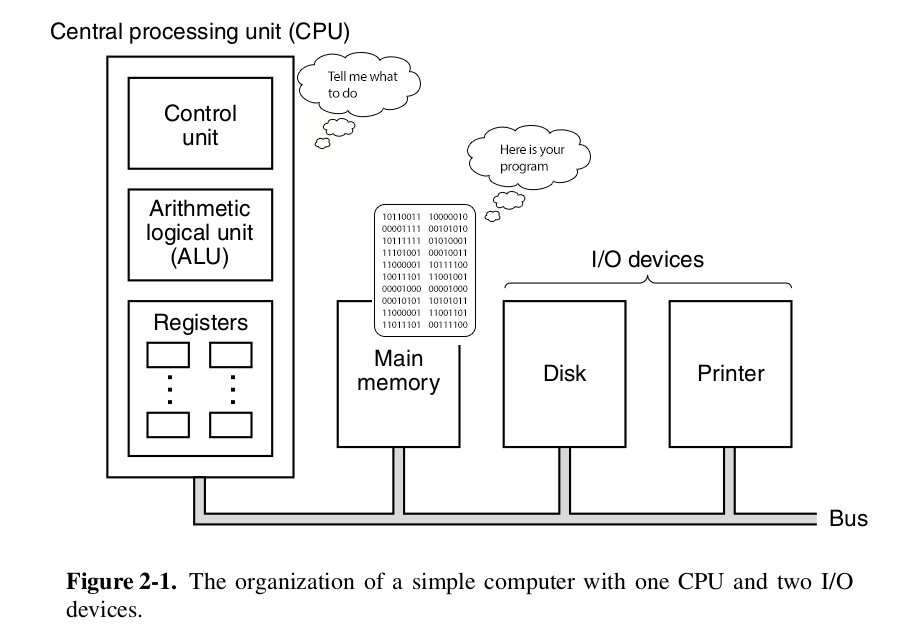
\includegraphics[width=80mm]{images/computer2.png}

    \end{columns}
\end{frame}

\begin{frame}{La computadora: Un sistema complejo}{CHIP}

    \begin{columns}[onlytextwidth,T]
      \column{\dimexpr\linewidth-60mm-5mm}

	\begin{itemize}
	\begin{small}
\bigskip
  \item[Chip] Die en inglés, es empaquetado dentro de un componente que permite su utilizacióin mecánica en un PCB.

\bigskip
\item[Densidad] La tecnología que se utiliza para fabricar los chips (dies), en los circuitos integrados, es el trasistor CMOS.\\
Actualmente la densidad es tan grande que existen miles de millones de transistores en un unico chip.

	\end{small}
	\end{itemize}

      \column{60mm}
    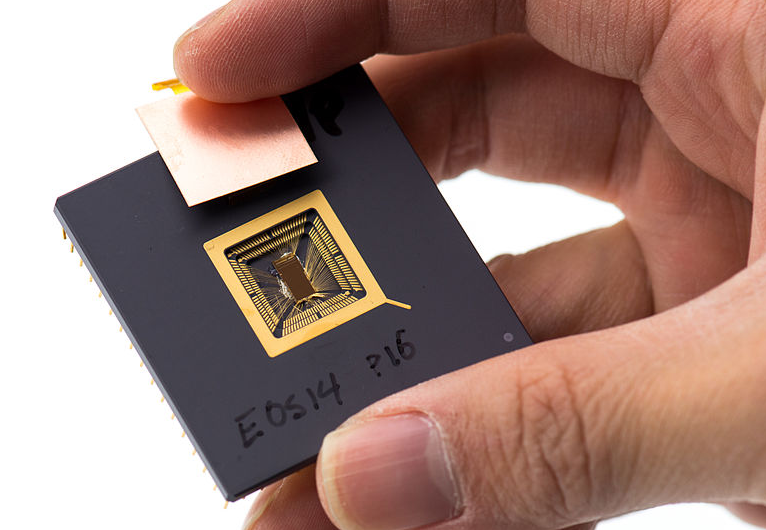
\includegraphics[width=80mm]{images/chip.png}

    \end{columns}
\end{frame}




\begin{frame}{La computadora: Un sistema complejo}{CHIP Barcelona}

    \begin{columns}[onlytextwidth,T]
      \column{\dimexpr\linewidth-60mm-5mm}

	\begin{itemize}
	\begin{small}
\bigskip
  \item[Chip] Die en inglés, es empaquetado dentro de un componente que permite su utilizacióin mecánica en un PCB.

\bigskip
\item[Densidad] La tecnología que se utiliza para fabricar los chips (dies), en los circuitos integrados, es el trasistor CMOS.\\
Actualmente la densidad es tan grande que existen miles de millones de transistores en un unico chip.

\bigskip
\item[Barcelona] Un microprocesador de 4 cores

	\end{small}
	\end{itemize}

      \column{50mm}
    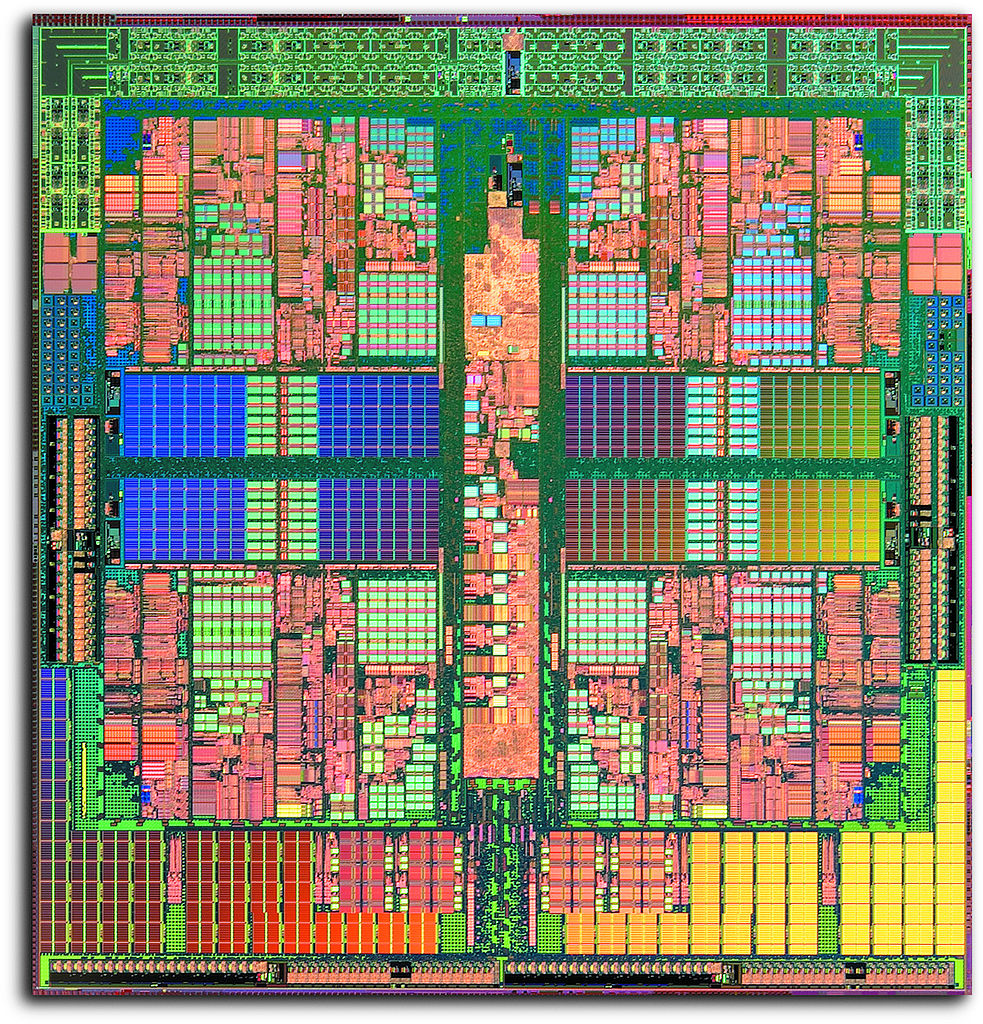
\includegraphics[width=80mm]{images/barcelona.png}

    \end{columns}
\end{frame}


\begin{frame}{La computadora: Un sistema complejo}{Transistor CMOS}

    \begin{columns}[onlytextwidth,T]
      \column{\dimexpr\linewidth-60mm-5mm}

	\begin{itemize}
	\begin{small}
\bigskip
  \item[Compuertas] Con circuitos CMOS se fabrican compuertas, que pueden operar digitalmente y realizar una simple función lógica.

\bigskip
\item[NOT] Una compuerta NOT (circuito básico CMOS) se puede fabricar utilizando dos transistores MOS complementarios.

	\end{small}
	\end{itemize}

      \column{50mm}
    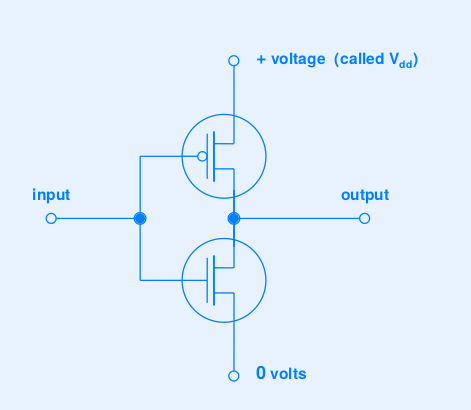
\includegraphics[width=50mm]{images/cmos2.png}

    \end{columns}
\end{frame}



\subsection{Abstracciones en la computadora}


\begin{frame}{La computadora: Un sistema complejo}

    \begin{columns}[onlytextwidth,T]
      \column{\dimexpr\linewidth-60mm-5mm}

	\begin{itemize}
	\begin{small}
\bigskip
  \item[Abstracción] El hardware y software de una computadora
consiste de una jerarquía en capas, donde cada capa de hardware o software
le oculta detalles a la capa superior.

\bigskip

\item[Principio] \textit{El principio de abstracción} es el que \textit{permite}
a los diseñadores de hardware y software poder \textit{entender la complejidad} 
de los sistemas de cómputo que construyen.

\bigskip

\item [Interfaz] EL nivel \textit{Arquitectura del Conjunto de 
Instrucciones (ISA)}, es la interfaz entre el hardware y el software.

	\end{small}
	\end{itemize}

      \column{60mm}
    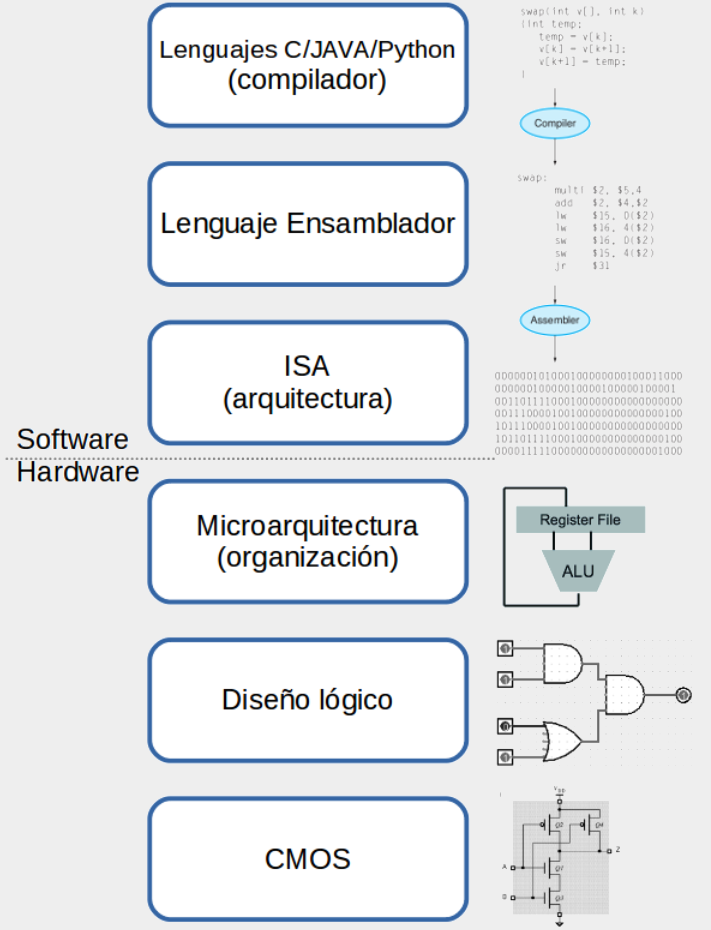
\includegraphics[width=50mm]{images/abstracciones2.png}

    \end{columns}

\end{frame}



\begin{frame} {Diseño lógico} {La computadora: Un sistema complejo}

    \begin{columns}[onlytextwidth,T]
      \column{\dimexpr\linewidth-60mm-5mm}

	\begin{itemize}
	\begin{small}
\bigskip
  \item[Boole] El diseño lógico (o diseño digital), es actuamente realizado utilizando el algebra de Boole (también llamado algebra de switching)

\bigskip
  \item[SFM] Las máquinas de estado finito pueden ser esquematizadas con diseño digital, y permiten diseñar máquinas algoritmicas.
\bigskip

	\end{small}
	\end{itemize}

      \column{60mm}
    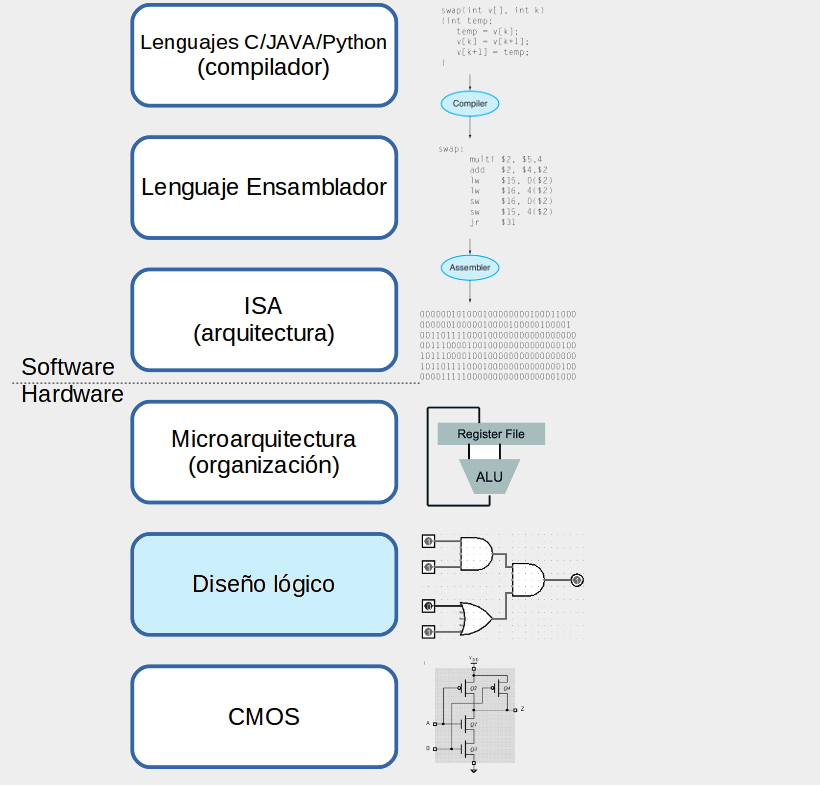
\includegraphics[width=65mm]{images/dis_logico.png}

    \end{columns}

\end{frame}





\subsection{Terminología: Arquitectura y Organización de un procesador}

\begin{frame} {Organización de una computadora} {La computadora: Un sistema complejo}

  \footnotesize{Es el diseño e implementación de la arquitectura (ISA) del microprocesador}

  \begin{columns}[onlytextwidth,T]
      \column{\dimexpr\linewidth-60mm-5mm}

	\begin{itemize}
	\begin{footnotesize}
\bigskip
\item[Micro] Hoy en día, a la organización de una computadora se la conoce como su \textbf{microarquitectura}

\bigskip
\item [Familia] Una arquitectura puede tener muchas organizaciones diferentes. 


\bigskip
\item [Ortogonales] La arquitectura y la organización son ortogonales; es decir, son totalmente independientes


	\end{footnotesize}
	\end{itemize}
\bigskip
\footnotesize{La \textbf{\textit arquitectura} especifica lo \textbf{\textit que} puede hacer una computadora y la \textbf{\textit organización} especifica \textbf{\textit cómo} lo hace.}

      \column{60mm}
	\bigskip
    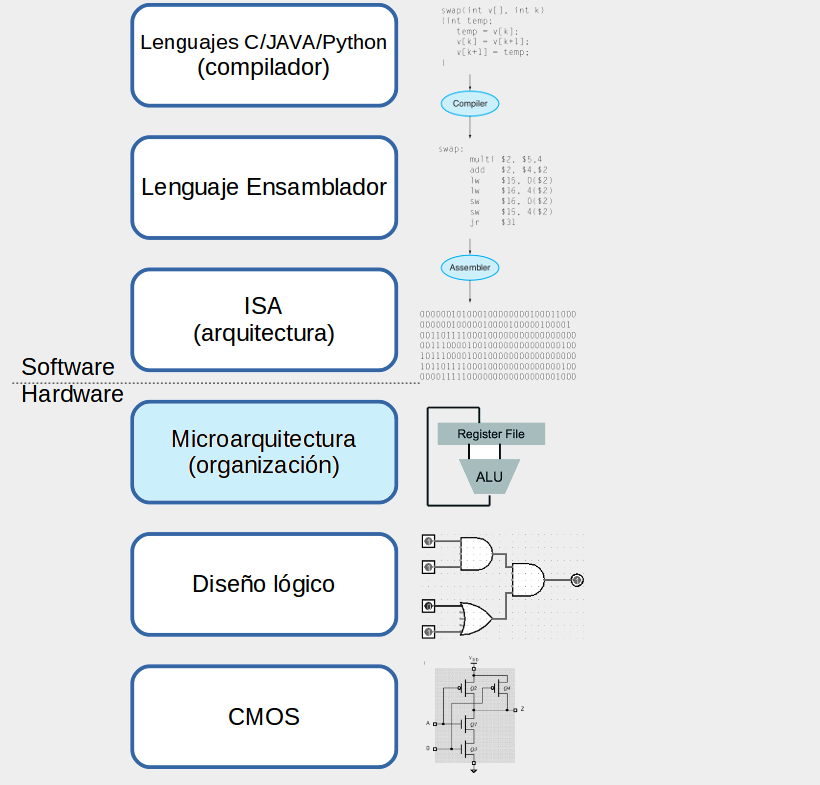
\includegraphics[width=65mm]{images/microarquitectura.png}

    \end{columns}

\end{frame}


\begin{frame}{Arquitectura de una computadora}{La computadora: Un sistema complejo}

  \footnotesize{Es la descripción del lenguaje máquina de una computadora \\(arquitectura del conjunto de instrucciones o ISA)}

  \begin{columns}[onlytextwidth,T]
      \column{\dimexpr\linewidth-60mm-5mm}

	\begin{itemize}
	\begin{footnotesize}

\bigskip
\item[Modelo] La arquitectura del conjunto de instrucciones define el modelo de programación.

\bigskip
\item[Abstracción] La arquitectura es una entidad abstracta, porque no considera detalles específicos del diseño o implementación.


\bigskip
\item[Componentes] La arquitectura (ISA) está compuesta por el conjunto de registros, el conjunto de instrucciones y los modos de direccionamiento.

\bigskip
\item[Interfaz] El lenguaje ensamblador de una computadora es una abstracción de la arquitectura

	\end{footnotesize}
	\end{itemize}

      \column{60mm}
    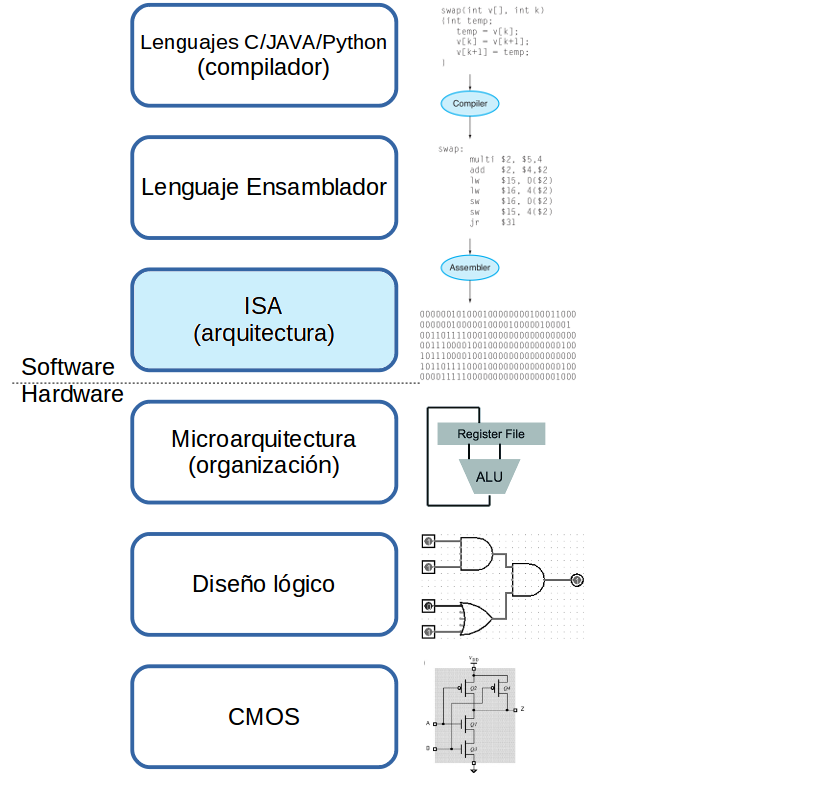
\includegraphics[width=65mm]{images/arquitectura.png}

    \end{columns}

\end{frame}


%     ibm 360 (mainframe), cray1 (supercoputaodra)
%     pdp-11 (creacion de unix) (minicomputadora)
%     4004 primer chip integrado
%     apple II y ibm pc (computadora personal)
%     open mobile komunications (smartphones)
%     iphone smartphone


\subsection{Historia: Eras tecnológicas, avances, y limitaciones}

\begin{frame} {Algunas computadoras importantes en la Historia}{ENIAC} 

    \begin{columns}[onlytextwidth,T]
      \column{\dimexpr\linewidth-50mm-5mm}


    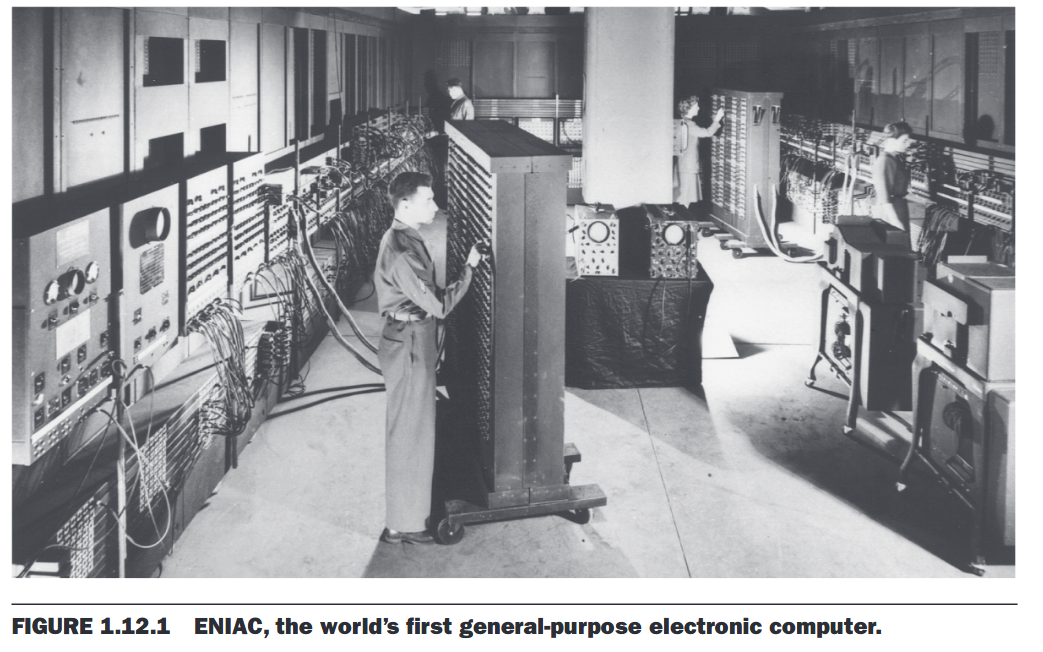
\includegraphics[width=100mm]{images/eniac.png}


    \end{columns}

\end{frame}





\begin{frame} {Algunas computadoras importantes en la Historia}{UNIVAC} 

    \begin{columns}[onlytextwidth,T]
      \column{\dimexpr\linewidth-50mm-5mm}


    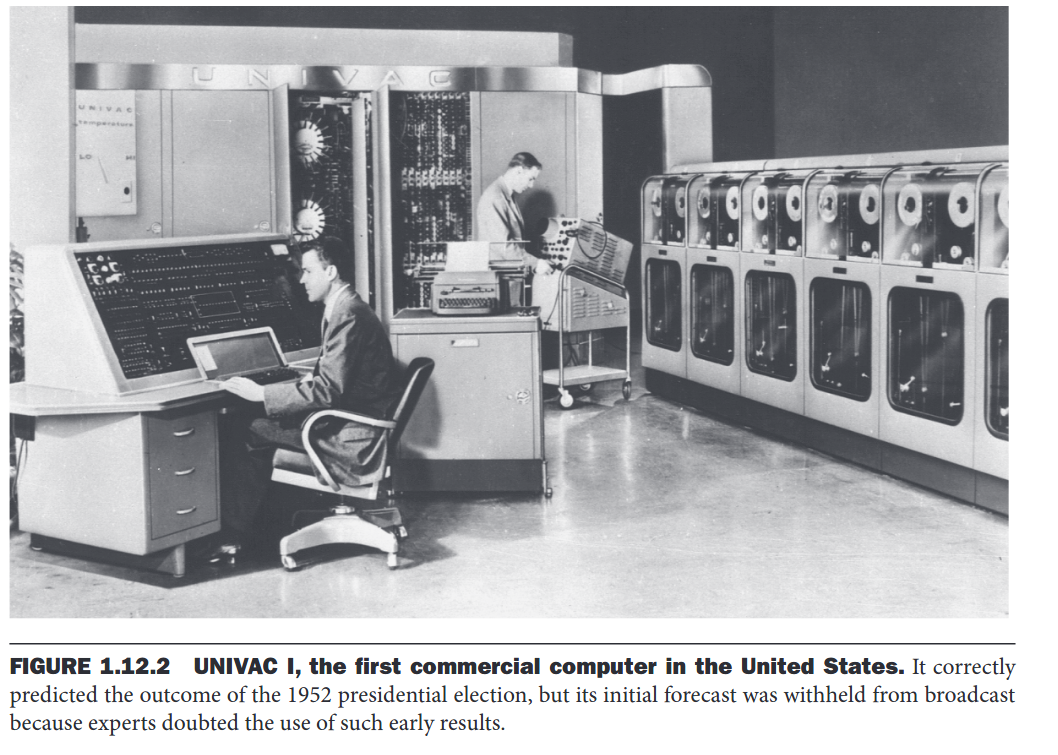
\includegraphics[width=100mm]{images/univac.png}


    \end{columns}

\end{frame}


\begin{frame} {Algunas computadoras importantes en la Historia}{IBM 360} 

    \begin{columns}[onlytextwidth,T]
      \column{\dimexpr\linewidth-40mm-5mm}

	\begin{itemize}
	\begin{footnotesize}
  \item El \textbf{IBM S/360 (S/360)} fue la primer familia de computadoras, lanzada en 1964,
compuesta de computadoras grandes y 
pequeñas, a diferentes precios y rendimientos; pero 
\textbf{todas de la misma arquitectura}.

\item Esto permitía a los clientes usar modelos más baratos y después ampliarlos a sistemas más potentes conforme se incrementaban sus necesidades.

\item IBM hizo el primer uso comercial de la tecnología de micro código para lograr esta compatibilidad.

    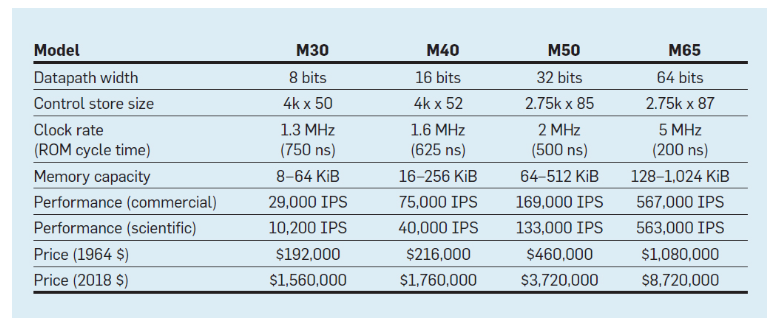
\includegraphics[width=70mm]{images/360-versions.png}


	\end{footnotesize}
	\end{itemize}

      \column{40mm}
    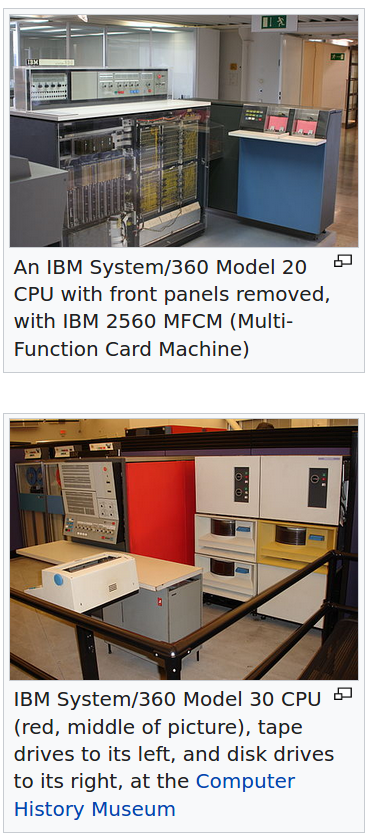
\includegraphics[width=30mm]{images/360.png}

    \end{columns}

\end{frame}



\begin{frame} {Algunas computadoras importantes en la Historia}{IBM 360} 

    \begin{columns}[onlytextwidth,T]
      \column{\dimexpr\linewidth-50mm-5mm}


    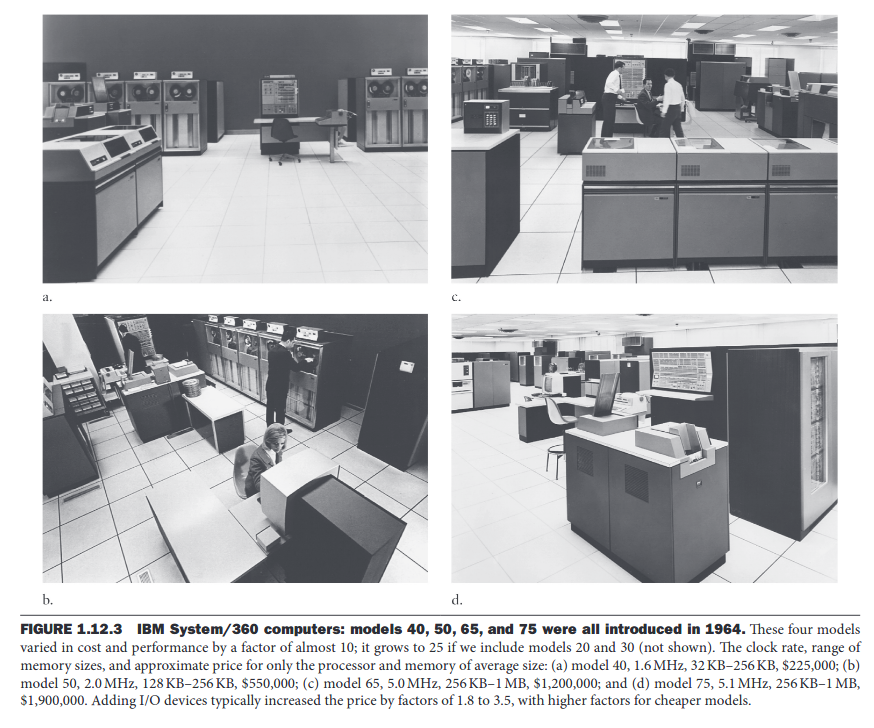
\includegraphics[width=100mm]{images/3602.png}


    \end{columns}

\end{frame}




\begin{frame} {Algunas computadoras importantes en la Historia}{4004} 

    \begin{columns}[onlytextwidth,T]
      \column{\dimexpr\linewidth-50mm-5mm}

	\begin{itemize}
	\begin{footnotesize}
  \item El \textbf{Intel 4004 (i4004)}, 
fue el primer microprocesador en un sólo chip, lanzado en 1971.
\bigskip
\item Estaba construído con aproximadamente 2500 transistores, e inició la era de los microprocesadores y Sillicon Valley.

\bigskip
    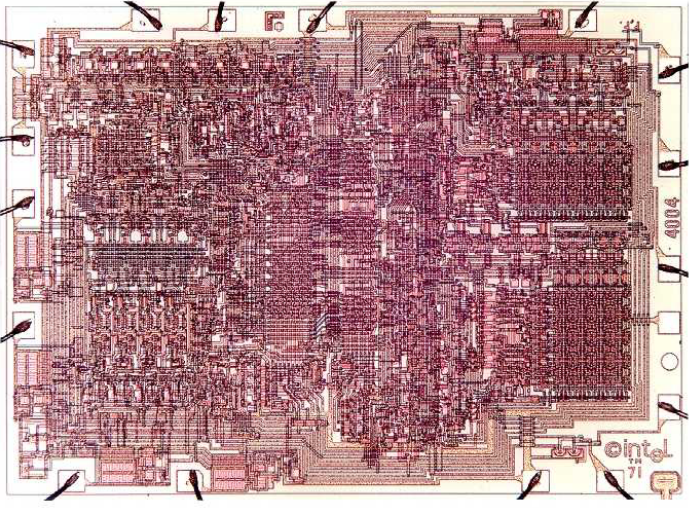
\includegraphics[width=50mm]{images/4004.png}

\tiny{(foto del interior del chip 4004)}

	\end{footnotesize}
	\end{itemize}

      \column{40mm}
    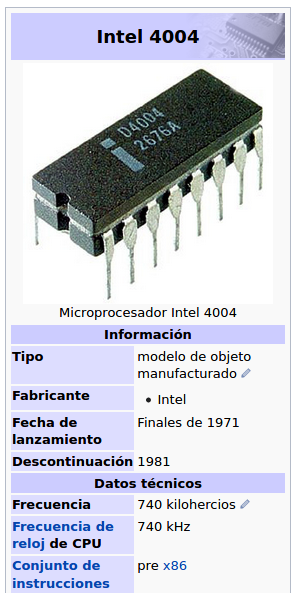
\includegraphics[width=30mm]{images/4004-2.png}

    \end{columns}

\end{frame}



\begin{frame} {Algunas computadoras importantes en la Historia}{Cray-1} 

    \begin{columns}[onlytextwidth,T]
      \column{\dimexpr\linewidth-50mm-5mm}

	\begin{itemize}
	\begin{footnotesize}
  \item El \textbf{Cray-1} fue una supercomputadora diseñada por varios ingenieros, 
encabezados por Seymour Cray para Cray Research. 
\bigskip

\item El primer sistema Cray-1 fue instalado en el laboratorio nacional de Los Álamos en 1976. 

\bigskip
\item Es uno de las supercomputadores más conocidas y exitosas de la historia, y de las más potentes en su época. 

	\end{footnotesize}
	\end{itemize}

      \column{40mm}
    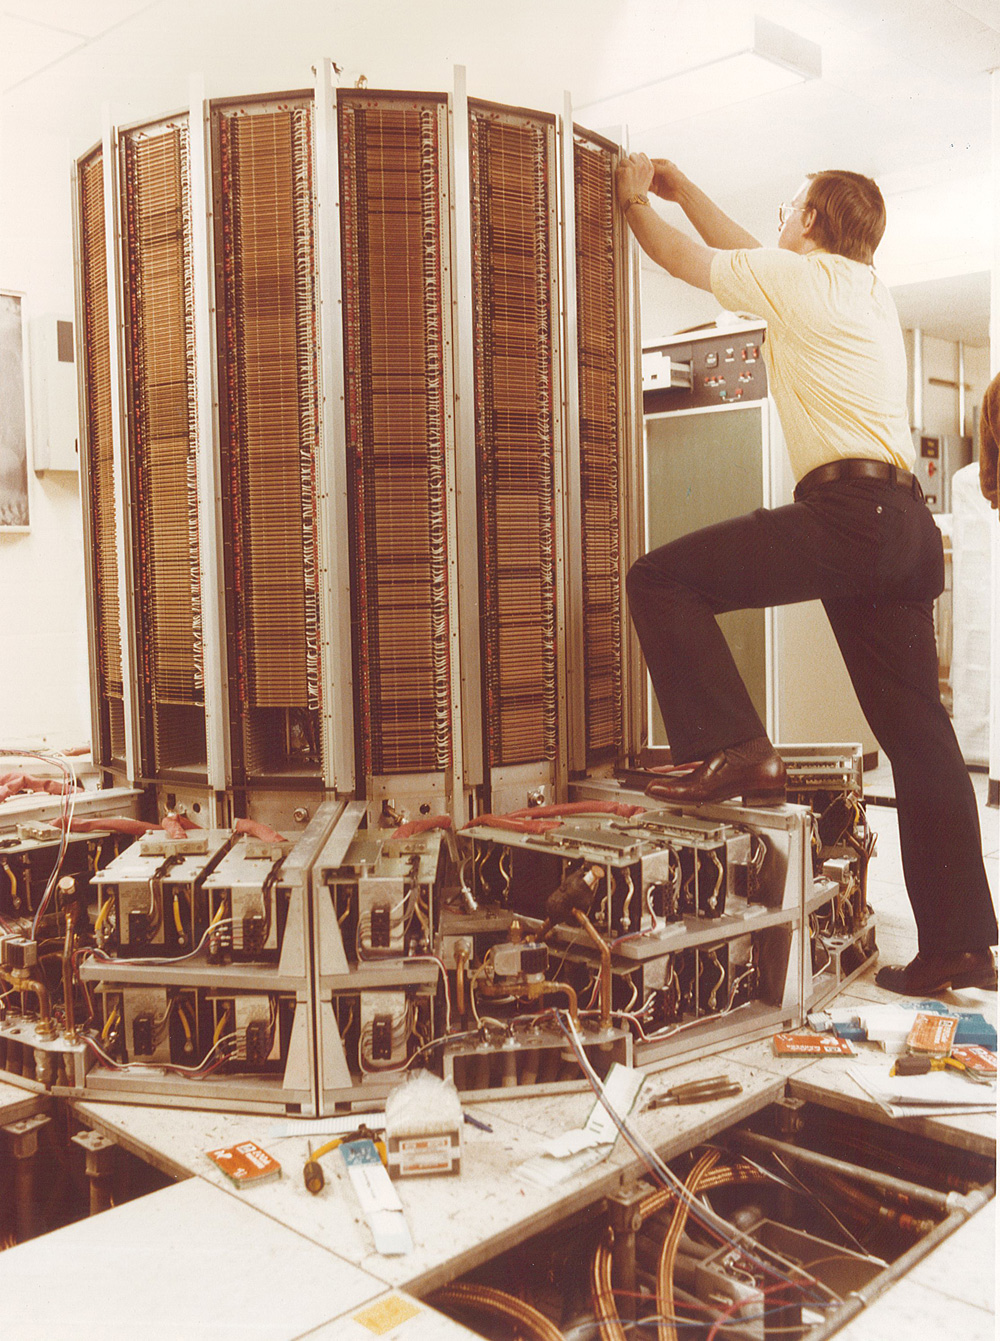
\includegraphics[width=40mm]{images/cray1.png}

    \end{columns}

\end{frame}





\begin{frame} {Algunas computadoras importantes en la Historia}{Apple II} 

    \begin{columns}[onlytextwidth,T]
      \column{\dimexpr\linewidth-50mm-5mm}

	\begin{itemize}
	\begin{footnotesize}
  \item La familia de computadores \textbf{Apple II} fue la primera serie de microcomputadoras de producción masiva, fabricada por Apple Computer en 1977.

\bigskip
\item El Apple II tenía una arquitectura de 8 bits basada en el procesador 6502.

\bigskip
\item Al igual que la Apple I, la Apple II fue diseñada por Steve Wozniak.

	\end{footnotesize}
	\end{itemize}

      \column{50mm}
    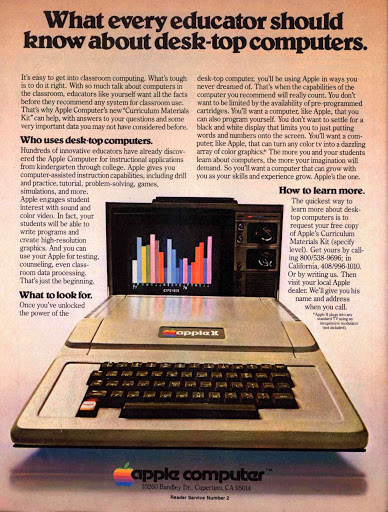
\includegraphics[width=50mm]{images/apple22.png}

    \end{columns}

\end{frame}


\begin{frame} {Algunas computadoras importantes en la Historia}{IBM PC} 

    \begin{columns}[onlytextwidth,T]
      \column{\dimexpr\linewidth-50mm-5mm}

	\begin{itemize}
	\begin{footnotesize}
  \item El \textbf{IBM Personal Computer (IBM PC)}
es la versión original y el progenitor de la plataforma de hardware compatible IBM PC, lanzado en 1981.
\bigskip
\item El IBM PC tenía una arquitectura de 16bits basado en un microprocesador Intel 8088 (con un bus de 8bits). 

\bigskip
\item El IBM PC es el predecesor de las actuales computadoras personales y progenitor de la plataforma compatible IBM PC. 

	\end{footnotesize}
	\end{itemize}

      \column{50mm}
    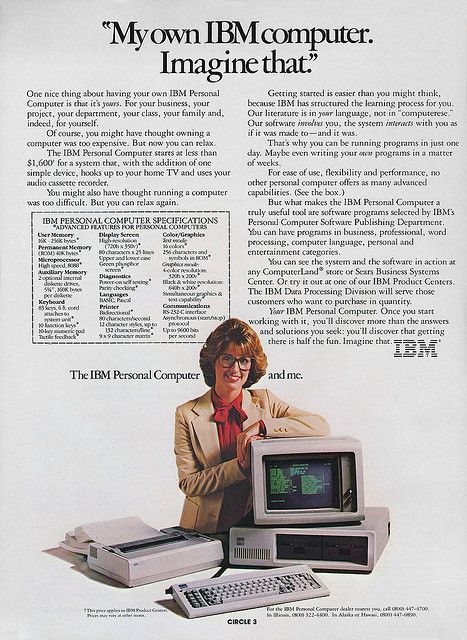
\includegraphics[width=50mm]{images/ibmpc.png}

    \end{columns}

\end{frame}


\begin{frame} {Eras tecnológicas} 

    \begin{columns}[onlytextwidth,T]
      \column{\dimexpr\linewidth-60mm-5mm}

	\begin{itemize}
	\begin{small}
\bigskip
  \item Electromecánicos

\bigskip
  \item Relés
\bigskip
  \item Tubos de vacío
\bigskip
  \item Transistor
\bigskip
  \item Circuitos integrados (CMOS)

	\end{small}
	\end{itemize}

      \column{60mm}
    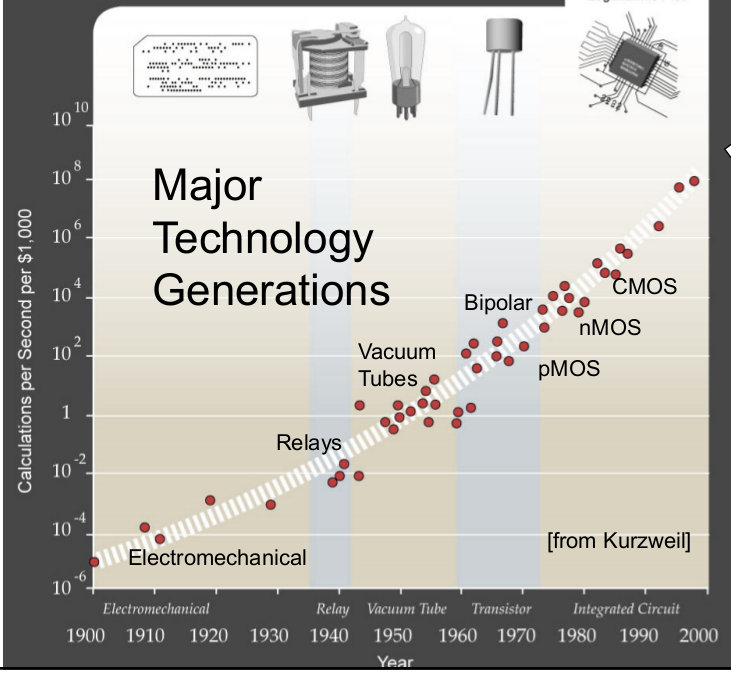
\includegraphics[width=65mm]{images/eras.png}

    \end{columns}

\end{frame}



\begin{frame} {Avances tecnológicos} 

    \begin{columns}[onlytextwidth,T]
      \column{\dimexpr\linewidth-50mm-5mm}

	\begin{itemize}
	\begin{small}

\bigskip
  \item[Tecnológicos] El incremento de transistores que anualmente pudieron incorporarse en un chip significó una mejora de rendimiento del 23\%.

\bigskip
  \item[Microarquitectura] Los avances en la Organización del procesador han producido grandes mejoras en la performance.
	\end{small}
	\end{itemize}

      \column{60mm}
    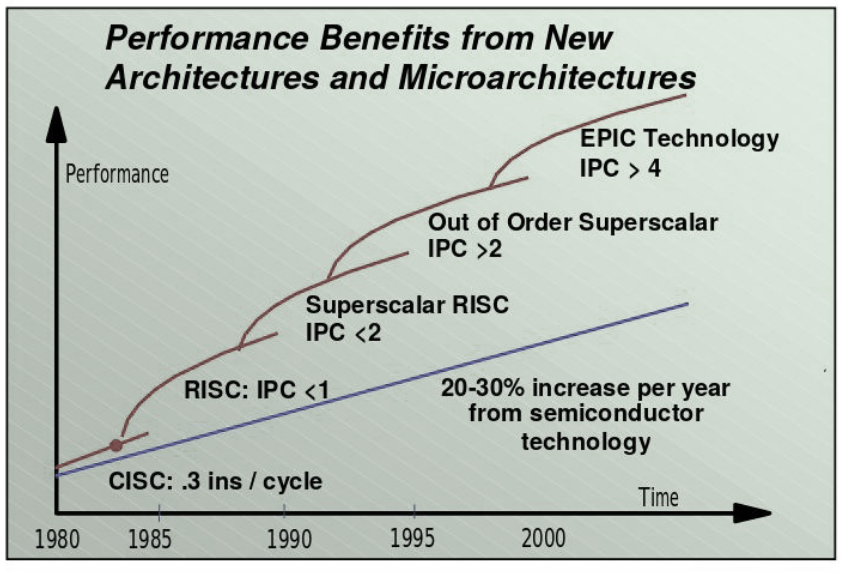
\includegraphics[width=60mm]{images/mejoras-arq-org.png}

    \end{columns}

\end{frame}



\subsection{Tiempo de ejecución (rendimiento)}
\subsection{MIPS/RISCV ISA (Arquitectura de una computadora real)}



\subsection{Recursos}

\begin{frame}[fragile]
  \frametitle{Recursos de la materia}

\begin{small}
\begin{itemize}

\item Web: \footnotesize{\texttt http://se.fi.uncoma.edu.ar/ayod1c/}\\
(se alcanza también desde la materia en PEDCO).

\item FOROs de PEDCO (Novedades y Consultas)
\item Telegram (para consultas)
\item Google meet para las exposiciones y discuciones temáticas online\\ (se darán los enlaces de encuentros en las clases).
\item Bibliografía:

\begin{itemize}

\item Andrew S. Tanenbaum (2000), ORGANIZACIÓN DE COMPUTADORAS un enfoque estructurado, Editorial Prentice Hall. (10 copias en biblioteca)
\item David. Patterson, John L. Hennessy, ORGANIZACIÓN Y DISEÑO DE COMPUTADORES La interfaz hardware/software, McGraw-Hill (8 copias en biblioteca).
\item Apuntes y artículos en la web de la materia
\item David. Patterson, John L. Hennessy, Computer Organization and Design RISC-V Edition 1st Edition The Hardware Software Interface. ISBN: 9780128122754

\end{itemize}

\end{itemize}
\end{small}

\end{frame}


\end{document}

%%% Local Variables:
%%% mode: latex
%%% TeX-master: t
%%% TeX-engine: xetex
%%% End:
